\documentclass[oneside,senior,etd]{BYUPhys}

\usepackage[utf8]{inputenc}
\usepackage{rotating} 

\usepackage[english, russian]{babel}
\usepackage{listings}
\usepackage{amsfonts} % Пакеты для математических символов и теорем
\usepackage{amstext}
\usepackage{amssymb}
\usepackage{amsthm}
\usepackage{graphicx} % Пакеты для вставки графики
\usepackage{subfig}
\usepackage{color}
\usepackage[unicode]{hyperref} 
\usepackage[nottoc]{tocbibind} % Для того, чтобы список литературы отображался в оглавлении
\usepackage{algorithmic} % Для записи алгоритмов в псевдокоде
\usepackage{algorithm}
\usepackage{verbatim} % Для вставок заранее подготовленного текста в режиме as-is
\usepackage{indentfirst}

\usepackage{tikz} 
\usetikzlibrary{shadows,arrows}

\Chair{Кафедра алгоритмических языков}
\Lab{~}
\Year{2018}
  \Month{}
  \City{Москва}
  \AuthorText{Автор}
  \Author{Шавалиева Ралина Забировна}
  \AuthorEng{}
  \AcadGroup{425}

  \TitleTop{Автоматическое извлечение гиперонимов}
  \TitleBottom{из больших текстовых корпусов.} % leave empty if you don't need it
  \TitleTopEng{Development of iterative algorithms for searching}
  \TitleBottomEng{automorphisms and isomorphisms of combinatorial objects.} % leave empty if you don't need it  
  \docname{ВЫПУСКНАЯ КВАЛИФИКАЦИОННАЯ РАБОТА}
  \Advisor{должность???
  
  Лукашевич Наталья Валентиновна}  
  \AdvisorDegree{}



%%%% DON'T change this. It is here because .sty does not support cyrillic cp properly %%%%
\University{Московский государственный университет имени М.В.Ломоносова}
\Faculty{Факультет вычислительной математики и кибернетики}
\GrText{группа}
\AdvisorText{Научный руководитель}

\begin{document}
\fixmargins
\makepreliminarypages

\oneandhalfspace

\tableofcontents

\section*{Введение}
\addcontentsline{toc}{section}{Введение}
\label{sec:Introduction} \index{Introduction}
\large 

В наше время компьютерная обработка естественного языка является одной из самых
востребованных областей искусственного интеллекта. Для того, чтобы правильно
распознать смысл фразы, написанной человеком, необходимо иметь дополнительные
знания о каждом слове этого предложения и существующих связей между ними. К такой
вспомогательной информации относится отношение \textit{is-a}, что означает отношение
обобщения.

Способность к обобщению лежит в основе человеческого познания. Люди без труда могут
заменить частное на общее. Например, слово <<кошка>> на слово <<животное>>,
<<автомобиль>> на <<транспорт>>, <<красный>> на <<цвет>>. Для каждой пары общее слово имеет
термин \textit{гипероним}, а частное - \textit{гипоним}. Для каждого гипонима может существовать
несколько гиперонимов, и наоборот.


\begin{figure}[ht]
\centering 
    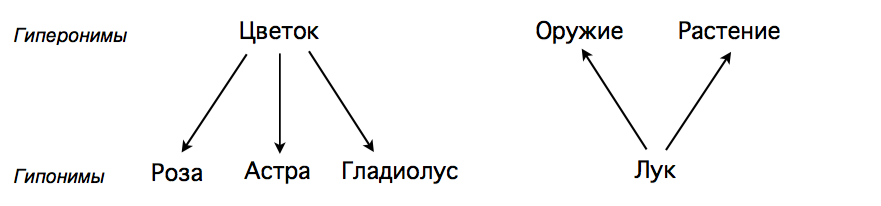
\includegraphics[scale=0.6]{image/Example.png}
    \caption{Пример связи гипонимов с гиперонимами.}
    \label{srg}
\end{figure}



Способность успешного распознавания таких лингвистических отношений приносит вклад
в такие области, как вопросно-ответная система, системы семантического поиска,
управление записями (система хранения и отслеживания документов), а также
информационный поиск и навигация по сайтам.

Например, наличие информации, что слова <<гепард>> и <<животное>> связаны отношением
\textit{is-a}, может помочь при ответе на вопрос <<какое самое быстрое животное?>>. А система
информационного поиска сможет подобрать соответствующие сайты, при получении
такого же запроса.

В добавок, отношение гипоним-гипероним - это основа почти любой семантической сети и
таксономии (иерархической системы отношений сущностей определенной области
знаний). Наличие таких построенных структур, помогает при реферировании текста, т.е.
извлечении из него основного содержания или заданной информации с целью
письменного изложения.

Таким образом, проблема определения отношений обобщения весьма актуальна как в
области лингвистики, так и в области искусственного интеллекта.

На данный момент большинство ресурсов, позволяющих определять отношение
обобщения, написаны вручную, что очень дорого в плане их создания и поддержки в
актуальном состоянии. Ручные словари зачастую имеют не достаточно большую область
покрытия. К тому же, в большинстве случаев, нет возможности выставления вероятности
наличия связи непрерывной случайной величиной от 0 до 1, а лишь только дискретная
степень допустимости существования отношения. Например, 0 - нет связи, 1- слабая, 2 -
средняя, 3 - сильная. Таким образом, нет возможности определить, какое из слов в
качестве гиперонима подходит больше, если есть несколько кандидатов имеющих
одинаковую степень. Для современных задач, появляется необходимость создания
автоматической системы поиска связи гипоним-гипероним.

Существует два основных вида постановки задачи. Первая, наиболее распространенная,
это сопоставление каждой паре слов 1 или 0, в зависимости от того, есть связь или нет.
Такого рода задача бинарной классификации неоднократно подвергалась критике за её
чрезмерную простоту, а также из-за невозможности сравнения кандидатов, как и в случае
ручных словарей. Второй способ заключается в поиске гиперонимов, т. е. предоставлении
ранжированного списка слов, которые наиболее вероятно являются гиперонимами
заранее заданному гипониму. Поиск таких слов происходит из конкретного словаря,
приближенному к словарю всех слов и устойчивых выражений для определенного языка.

В данной работе исследуется второй вид постановки задачи - поиск гиперонимов.
Рассматриваются различные алгоритмы, как с применением машинного обучения, так и
основанные на текстовых шаблонах. И производится сравнение полученных результатов
по различиям метрикам качества.





 % введение
\section{Постановка задачи}
\label{sec:Chapter_1} \index{Chapter_1}
\large

Целью данной работы является реализация различных алгоритмов извлечения
гиперонимов из текстовых корпусов. Исследовать алгоритм, основанный на анализе
текстов средством рукописных регулярных выражений, а также класс алгоритмов,
использующих разные виды нейронных сетей, с последующим обучением на размеченных
данных.

Алгоритм должен для заданного гипонима составлять упорядоченный по вероятности
список гиперонимов.\\



\textbf{ЗАДАЧИ}

\begin{enumerate}
\item Исследование существующих подходов к решению поставленной задачи
\item Выбор набора данных. Разделение его на обучающую и тестовую части.
\item Выбор метрик оценки качества модели. Метрики должны учитывать порядок выбранных гиперонимов, так как
основная задача – ранжирование списка.
\item Построение и тестирование модели, основанной на рукописных шаблонах
\item Исследование первой модели векторного представления слов, основанной на гипотезе
дистрибутивной семантики. \textit{PPMI} + \textit{SVM}.
\item Построение моделей, использующих различные комбинации векторов, полученных
алгоритмом Word2Vec. Дообучение алгоритмом \textit{GBR} и LambdaRank.
\item Реализация нейронной сети, разделяющей каждое слово на 2 вектора: слово в
качестве гипонима и слово в качестве гиперонима. Распараллеливание алгоритма
средствами Hadoop MapReduce.
\item Сравнение результатов, полученных всеми построенными моделями. Определение лучшей модели.
\item Тестирование выбранной модели на полных данных.
\end{enumerate}

 % постановка задачи
\section{Обзор существующих алгоритмов}
\label{sec:Chapter_2} \index{Chapter_2}
\large

\subsection{Модель, основанная на лексико-синтаксических шаблонах}

Данный метод был разработан профессором Марти Херст в 1992 году \cite{hearst1992}. Алгоритм является
одним из первых в области автоматического определения отношения обобщения между
словами. Считается, что пара слов в предложении связана отношением гипоним-гипероним, если она удовлетворяет одному из шаблонов, например, таких, как:

\begin{itemize}
\item $[A]$ for example $[B]$ - например
\item $[A]$ such as $[B]$ - такие как
\item $[A]$ include $[B]$ - включая
\item $[A]$ especially $[B]$ - особенно
\end{itemize}

Здесь $[A]$ обозначает \textit{гипероним}, а $[B]$ - список \textit{гипонимов}. Например, <<I like flowers, such as
roses or peonies>> - <<мне нравятся цветы, такие как розы или пионы>>. В данном случае в
качестве гиперонима выступает слово <<цветы>>, а гипонимы - <<розы>> и <<пионы>>.

Список таких словосочетаний не имеет фиксированного размера. Можно добавлять свои
примеры, подходящие конкретной области или исключать неподходящие.\\

\textbf{ПРЕИМУЩЕСТВА}

\begin{itemize}
\item Высокая точность
\end{itemize}

\textbf{НЕДОСТАТКИ}

\begin{itemize}
\item Главный недостаток такого подхода - низкая полнота определения связей. Необходим
очень большой текстовый корпус, чтобы выделить хотя бы базовые пары отношений.

\item Не каждый пример связи можно описать шаблоном.

\item Не улавливаются цепочки связей. То есть, если определены пары <<ласточка - птица>> и
<<птица - животное>>, то может не быть пары <<ласточка - животное>>.
\item Несмотря на высокую точность, встречаются случаи, когда пара слов неверно отмечена,
как имеющая связь is-a. Один из таких примеров пара предложений:

<<...\textbf{сities} in Asian countries such as \textbf{Tokyo} ...>> - <<... города в странах Азии, такие как Токио
...>>

<<...сities in Asian \textbf{countries} such as \textbf{Japan} ...>> - <<... города в странах Азии, таких как
Япония ...>>

В первом случае пара <<countries - Tokyo>> была бы отмечена неправильно

\item Для ранжирования гиперонимов недостаточно иметь только число, означающее сколько
раз встретилась конкретная пара, так как это зависит от конкретного текстового
корпуса.
\end{itemize}

\subsection{Векторное представление слов}

\subsubsection{Представление слов векторами, полученными при SVD разложении матрицы PPMI}

Данный подход основывается на предположении, которое называется
<<дистрибутивная гипотеза>>: лингвистические единицы, встречающиеся в схожих
контекстах, имеют близкие значения. Для такого подхода необходимо иметь достаточно
большой текстовый корпус.

Существует несколько способов получения контекстов для слова. Наиболее популярный
называется <<window-based>> метод. Задается величина ширины окна $k$. Далее
просматриваются все предложения, содержащие конкретное слово. К примеру,
интересующее нас слово $W_i$ находится в позиции $i$ в рассматриваемом предложении.
Контекстом данного предложения к $W_i$ будет набор слов ($W_{i-k}, \ldots W_{i-1}, W_{i+1}, \ldots W_{i+k}$) т.е $k$
слов, стоящих до $W_i$ и $k$ слов после. Величина окна произвольная, но чаще всего
выбирается от $2$ до $5$. Таким образом, для каждого слова строится набор его контекстов.

Исследовав схожесть наборов контекстов двух разных слов, можно судить об отношении
этих слов между собой. Например, в случае синонимов, наборы контекстов будут близки.
Задание же функции вычисления схожести является главным параметром таких моделей.

\textit{PPMI} (positive pointwise mutual information) - положительная поточечная взаимная
информация. Функция \textit{PPMI} является одной из оценок схожести двух лингвистических
единиц, например слов, контекстов, абзацев и т.п., на основе заданного текстового
корпуса. Для случая вычисления взаимной информации между словом и контекстом
данная функция задается следующей формулой:

$PPMI (w, c) = max(PMI (w, c), 0)$

$PMI (w, c) = \log \frac{p(w, c)}{p(w) \times p(c)}$, где


\begin{itemize}
\item $w$ - слово из текстового корпуса;

\item $c$ - контекст;

\item $p(w)$ - вероятность встречи слова $w$ в корпусе = частота появления слова в
корпусе, деленная на общее число слов

\item $p(c)$ - вероятность встречи данного контекста $c$ = частота появления контекста в
корпусе, деленная на общее число контекстов

\item $p(w,c)$ - вероятность встречи пары <<слово - контекст>> = частота появления
данной пары в корпусе, деленная на общее число пар

\end{itemize}

Таким образом, \textit{PPMI} вычисляется напрямую из текстового корпуса. Если слово и
контекст не связаны между собой, то 

$p(w, c) = p(w) \times p(c)$

и \textit{PPMI} для этой пары будет равно 0. Чем выше данный показатель, тем чаще слово $w$ появляется в сопровождении
контекста $c$.

Строится таблица $M$, строки которой соответствуют словам, а столбцы – контекстам.
Таблица заполняется соответствующими значениями \textit{PPMI}. Вектор слова определяется
величинами, расположенными в его строке. Длина вектора - количество найденных в
корпусе контекстов. Таким образом, схожесть наборов контекстов для двух слов
определяется близостью их векторов \cite{PPMI}.

Как можно заметить, величина встречаемости слова намного меньше размера множества
всех контекстов. Значит, матрица $M$ будет иметь большой размер, и при этом она будет
сильно разреженной. Возникает проблема <<проклятия размерности>>. 
Измерение
расстояния между такими векторами будет неинформативным, т.к согласно Закону
Больших Чисел, сумма разности каждого признака $n$ слагаемых стремится к некоторому фиксированному пределу при $n \to \infty$, следовательно, все точки
выборки становятся почти одинаково далеки друг от друга.

Одним из решений данной проблемы является снижение размерности алгоритмом \textit{SVD}
(Singular Value Decomposition). Данный алгоритм может приблизить матрицу $M$ размера $n \times m$, некоторой другой матрицей $M_k$ с заданным рангом $k$, такой, что её можно разложить в
произведение трех других матриц.

$M \approx M_k = U_k \times \Sigma_k \times V^T_k$,

где $U_k$ и $V_k$ - две унитарные матрицы, состоящие из левых и правых сингулярных
векторов соответственно

$V^T_k$ - это сопряжённо-транспонированная матрица к $V_k$;

$\Sigma_k$ — матрица размера $k \times k$ с неотрицательными элементами, у которой элементы,
лежащие на главной диагонали — это сингулярные числа (а все элементы, не лежащие на
главной диагонали, являются нулевыми)

Полученная матрица $U_k$ будет иметь размерность $n \times k$. Строки такой матрицы будут
соответствовать строкам исходной матрицы $M$, только размерность векторов изменится с
$m$ на $k$. Часть информации потеряется, но существенная её часть остается. Аналогично,
матрица $V^T_k$ несет информацию о столбцах матрицы $M$, только имея при этом меньший
размер.

Применительно к нашей задачи, разложение матрицы \textit{PPMI} приведет к получению
компактного векторного представления слов, сохраняющего информацию о контекстах.

Дальнейшая работа с полученными векторами будет описана в пункте 2.4.


\subsubsection{WORD2VEC}

Еще одним инструментом, реализующим модель векторного представления слов, является
Word2Vec. Этот инструмент был разработан группой исследователей Google в 2013 году,
под руководством Томаша Миколова.

\textit{Word2Vec} реализует две архитектуры - \textit{Continuous Bag-of-Words} (\textit{CBOW}) и \textit{Skip-gram}. Обе архитектуры построены на нейронных сетях и основаны на дистрибутивной гипотезе.

Принцип работы \textit{CBOW} — предсказание слова при данном контексте, а \textit{Skip-gram}
наоборот — предсказывает контекст при заданном слове. Независимо от архитектуры,
модель принимает в качестве входных параметров текстовый корпус, и формирует
векторное представление каждого слова, входящего в корпус и имеющего частотность в
заданном диапазоне.

Применяется искусственная нейронная сеть прямого распространения (Feedforward Neural
Network \cite{Feedforward}) с функцией активации иерархический софтмакс (Hierarchical Softmax \cite{SoftMax}) и/или
негативное сэмплирование (Negative Sampling \cite{NegSamp}). Метрика близости векторов – косинусное
расстояние.

Таким образом, данная модель позволяет получить еще одно векторное представление
каждого слова.

\subsubsection{Dynamic distance-margin model}

Две предыдущие модели позволили получить векторные представления слов,
основываясь на наборах их контекстов. При этом каждое слово учитывалось
только один раз, не было различия: слово выступает в качестве гипонима или в
качестве гиперонима.

Отношение is-a не является симметричным. Если пара слов $A-B$ связана
отношением гипоним-гипероним, то пара $B-A$ таким отношением уже не связана.
Более того, чем ближе вектор ${A}$ к вектору ${B}$, тем больше вероятность, что слова ${A}$ и ${B}$ являются синонимами. Необходимо подбирать границы близости: не слишком
далекие, чтобы слова имели связь друг с другом, и не слишком близкие, чтобы не
получать синонимичные пары. С точки зрения построения моделей, задача поиска
максимума или минимума решается проще и качественнее, чем определение таких
границ. Поэтому возникает предположение о разделение одного вектора слова на
два - вектор гипоним и вектор гипероним \cite{DDM}.

Вектор слова \textbf{$w$}, используемый, когда данное слово будет выступать в качестве
гипЕронима, обозначим за \textbf{$E(w)$}. Например, слово \textit{птица} в отношении (\textit{ласточка}, \textit{птица}). Когда в качестве гипОнима - за \textbf{$O(w)$}. Пример: в паре (\textit{птица}, \textit{животное}).

Предполагается, что построенная новая модель должна удовлетворять следующим
трем правилам:

\begin{enumerate}
\item Если пара слов $u-v$ связана отношением гипоним-гипероним, то вектора $O(u)$ и $E(v)$ находятся близко друг к другу. $O(u) \approx E(v)$.

\item Если пара слов $u-v$ являются ко-гипонимами, т.е. существует слово $w$,
являющееся гиперонимом, как для слова $u$, так и для слова $v$, то должно
выполняться соотношение $O(u) \approx O(v)$.

\item Аналогично, если пара слов является ко-гиперонимами, то должно быть верно: $E(u) \approx E(v)$.
\end{enumerate}

Таким образом задача сводится к минимизации расстояний $O(u) \approx E(v)$, $O(u) \approx O(v)$ и $E(u) \approx E(v)$.

В качестве обучающего множества берется набор триплетов $(u, v, q)$, где $u$ - гипоним, $v$ - гипероним, а $q$ - сколько раз пара гипоним-гипероним $(u, v)$ встретилась в текстовом корпусе. Такой набор данных может быть собран вручную или,
например, методом шаблонов, описанным в пункте 2.1. Необходимо учитывать, что
для получения хороших результатов, размер текстового корпуса должен быть
очень большим.

Для каждой пары $x = (u, v, q)$ из выбранного набора данных, вычисляется функция
расстояния между векторами $O(u)$ и $E(v)$. В качестве функции расстояния может,
например, выступать 1-норма разности векторов. Так

$f(x) = ||O(u) - E(v)||_1$

Для того, чтобы оценить величину ошибки модели на примере $x$, расстояние между
векторами слов $u$ и $v$ сравнивается с расстоянием от $u$ до произвольного слова $v'$.
Т.е выбирается негативный пример гиперонима для гипонима $u$. По
предположению, построенные вектора $O(u)$ и $E(v)$ должны быть ближе, чем
вектора $O(u)$ и $E(v')$. Насколько ближе они должны быть, определяется величинами $q$ и $q'$. Величина $q'$ означает, сколько раз пара гипоним-гипероним $(u, v')$
встретилась в текстовом корпусе. Так как слово $v$ выбирается случайным из всего
корпуса, то наиболее вероятно $q$ равняется нулю.

Величины $q$ и $q'$ показывают насколько вероятным может быть существование
отношения is-a между соответствующими им парами слов. Тогда, чем больше
разница этих вероятностей, тем расстояния между величинами $f(x)$ и $f(x')$ должно
быть больше. Учитывая проведенный анализ, вводятся следующие соотношения:

\begin{itemize}
\item $x' =$ \textit{триплет} $(u, v', q')$

\item $f(x) < f(x') - m(q, q')$

\item $m(q, q') = log(q + 1) - log(q' + 1) = log \frac{q + 1}{q' + 1}$
\end{itemize}


В таком случае, ошибку модели на примере $x$ можно вычислить как

$$max(0, f(x) - f(x') + m(q, q') )$$

И тогда модель будет обучаться уже на парах $(x, x')$.
Аналогично, в качестве негативного примера $x'$ может выступать не только триплет
$(u, v', q')$, но и $(u', v, q')$.

Для того, чтобы обучать модель чаще на парах, которые с большей вероятностью
имеют отношение is-a, используется искусственное увеличение обучающего
множества пар $(x, x')$ с учетом этой вероятности. Для каждого триплета $x$
подбирается столько негативных примеров $x'$, сколько раз $(u, v)$ встретилась в
текстовом корпусе, т.е создается $q$ различных пар $(x, x')$.
Итоговая функция потерь построенной модели вычисляется как:

$$\sum_{x = (u, v, q)} \sum_{j = 1}^{q} max(0, f(x) - f(x'_j) + m(x, x'_j))$$

При успешном обучении данной модели, она будет удовлетворять всем трем
условиям, описанным выше:

\begin{enumerate}
\item $O(u) \approx E(v)$ достигается за счет непосредственной минимизации расстояния $f(x)$
\item Если для пары $(u, v)$ существует слово $w$, являющееся гиперонимом, как для
слова $u$, так и для слова $v$, то из первого пункта следует: $O(u) \approx E(w)$ и $O(v) \approx E(w)$, а значит, и $O(u) \approx O(v)$. Другими словами, оба слова $u$ и $v$ подтягиваются к
слову $w$, тем самым становясь ближе друг к другу.
\item Аналогично достижима цель $E(u) \approx E(v)$
\end{enumerate}

Выполняя все эти 3 условия, становится возможным определение пары (\textit{ласточка,
животное}) имея в изначальном наборе данных только пары (\textit{ласточка, птица}) и
(\textit{птица, животное}). Устранился один из важных недостатков чисто шаблонных
моделей.

Обучение такой модели сводится к обучению нейронной сети, имеющей
следующую архитектуру:

\begin{figure}[H]
\centering 
    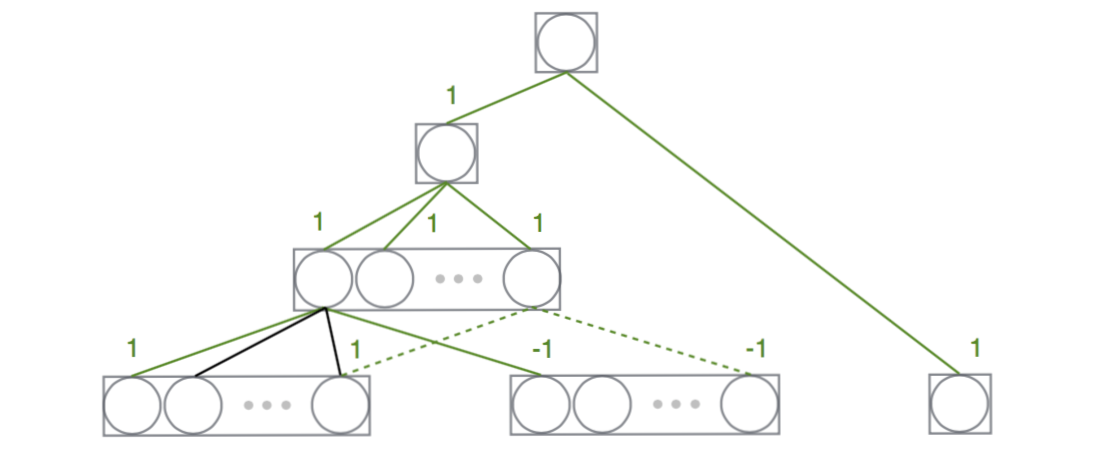
\includegraphics[scale=0.6]{image/NN_part1_new.png}
    \caption{$p(x)$ - вычисление расстояния между векторами $O(u)$ и $E(v)$ для $x = (u, v, q)$.}
    \label{srg}
\end{figure}

\begin{figure}[H]
\centering 
    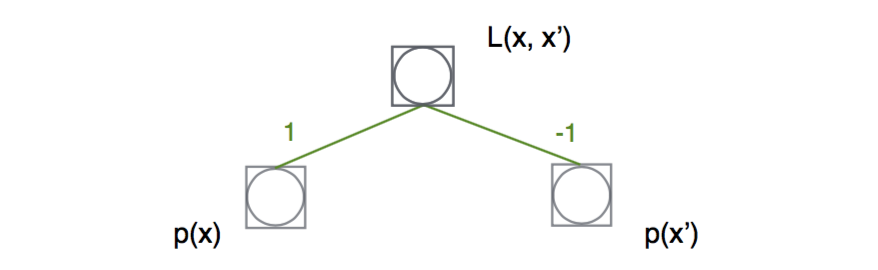
\includegraphics[scale=0.6]{image/NN_part2_new.png}
    \caption{$L(x, x’)$ - вычисление ошибки для триплета x и его негативного примера $x’$.}
    \label{srg}
\end{figure}

\begin{figure}[H]
\centering 
    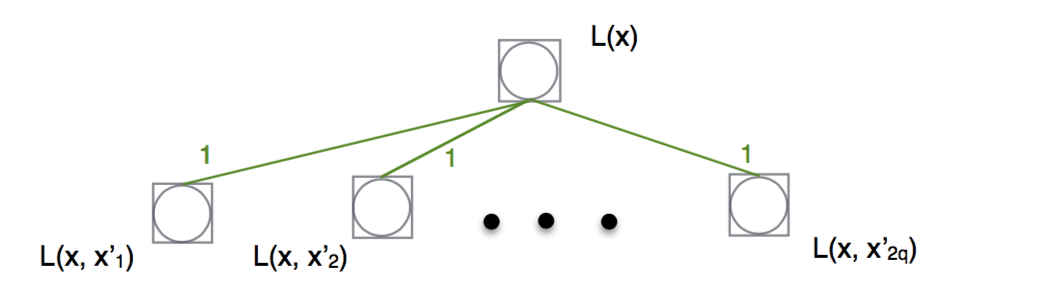
\includegraphics[scale=0.6]{image/NN_part3_new.png}
    \caption{$L(x)$ - вычисление суммарной ошибки для триплета $x$.}
    \label{srg}
\end{figure}

\begin{figure}[H]
\centering 
    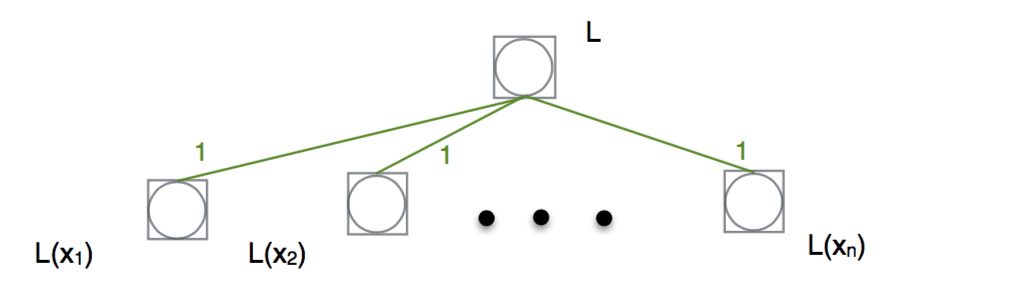
\includegraphics[scale=0.6]{image/NN_part4_new.png}
    \caption{$L$ - вычисление функции потерь модели.}
    \label{srg}
\end{figure}

Модель оптимизируется алгоритмом $SGD$.

Таким образом, разобраны три различные модели получений векторов слов.
Осталось рассмотреть способы вычисления итоговых предсказаний существования
отношений \textit{is}-a между словами, используя их векторное представление.



\subsubsection{Обучение модели, предсказывающей существование связи IS-A, на основе векторов слов.}

Как было сказано, большинство задач, связанных с темой определения
существования связи \textit{is}-a, были сведены к выставлению каждой паре слов либо 0
(связи нет), либо 1 (при её наличии). Поэтому чаще всего для последующего
обучения векторов был выбран алгоритм $SVM$.

Для обучения брался готовый размеченный корпус пар слов, имеющих между
собой отношение гипоним-гипероним, и подмешивался к нему набор пар, не
имеющих такой связи. Все, что оставалось, это скомбинировать вектора слов из
пары, в качестве входного вектора для обучения.

Существует множество различных комбинаций. Наиболее используемые из них
следующие:

\begin{itemize}
\item Разность векторов $<u - v>$
\item Соединение векторов (конкатинация) $<u, v>$
\item Вычисление косинусного расстояния $cos(u, v)$
\item Евклидово расстояние $|| u - v ||_2$
\item И их комбинации, например:
\begin{itemize}
\item конкатенация с добавлением евклидового расстояния

$<u, v, || u - v ||_2>$
\item разность векторов с добавлением косинусного расстояния

$<u - v, cos(u, v)>$
\end{itemize}
\end{itemize}

Таким образом для каждой из трех моделей получения векторного представления
слов, выбирался какой-то из способов комбинирования векторов и происходило
обучение на таких входных данных алгоритма $SVM$.

Как показали эксперименты, такие виды моделей давали показатели метрик
классификации лучше, по сравнению с чисто шаблонными методами. % определения и обозначения
\section{Описание тестовых данных и метрик оценки качества моделей}
\label{sec:Chapter_3} \index{Chapter_3}
\large


\subsection{Данные}

Для обучения и сравнения моделей, необходимо выбрать размеченный набор данных,
словарь, из которого будут выбираться подходящие гиперонимы, а также большой
текстовый корпус.

Все необходимые для данной задачи данные были предоставлены участникам конкурса
SemEval-2018 [ссылка].

\begin{enumerate}
\item Размеченный набор данных.

Для каждого из 1500 гипонимов, составлен эталонный ранжированный список
гиперонимов. Длина списка варьируется от 3 до 15 слов.

\item Словарь слов.

Предоставлен словарь, состоящий из 218755 слов. Только слова, включенные в
этот список могут быть взяты в качестве гиперонима

\item Текстовый корпус.

Для обучения своих моделей предоставлен UMBC корпус, содержащий в себе 3
миллиарда слов. Этот корпус составлен из отрывков веб страниц и является частью
Stanford WebBase Project. UMBC содержит в себе информацию многих различных
областей.
\end{enumerate}

Примеры данных находятся в приложении А.


\subsection{Метрики качества}

Так как главной задачей является извлечение и ранжирование гиперонимов, то были
выбраны метрики качества, учитывающие порядок слов в списке:

\begin{itemize}

\item Mean Reciprocal Rank (\textit{MRR}) - является показателем средней позиции первого правильно определенного гиперонима

$$MRR= \frac{1}{|Q|} \sum^{|Q|}_{i=1} \frac{1}{rank_i}$$

где $Q$ - множество гипонимов в тестовой выборке, а
$rank_i$ - позиция первого предсказанного гиперонима, который
есть в эталонном списке

\item Precision@k (P@k) - оценивает долю верно извлеченных гиперонимов в списке
слов, усеченном до $k$-й позициии.
$$P@k = \frac{1}{k} \sum^k_{i=1} isTrue(i)$$

где $isTrue(i) = 0$, если гиперонима, стоящего на $i$-й позиции в
предсказанном списке, нет в эталонном списке, и 1, если есть.
Для задачи данной работы, оценивается средняя величина $P@k$ $(ap@k)$ по всем гипонимам, где $k = 1, 3, 5$ и $15$

\item Mean Average Precision @15 (\textit{MAP}) - усредненная оценка $P@k$ по всем $k$ от $1$ до $15$

$$map@K = \frac{1}{N} \sum^N_{j=1} ap@K_j$$

\end{itemize}
 % описание алгоритма
\section{Исследование и построение решений задачи}
\label{sec:Chapter_4} \index{Chapter_4}
\large




\subsection{Шаблонный метод}

Для тестирования первого метода решения поставленной задачи, необходимо
было составить шаблоны поиска гипонимов и гиперонимов, аналогичных шаблонам
Марти Херст.

Были найдены уже готовые примеры шаблонов как в научных статьях, так и в
готовых программах, написанных на языке программирования. Наиболее широки
списком разнообразных шаблонов обладал класс \textit{hearstPatterns}, написанный на
языке Python. Всего в нем содержалось 48 примеров, написанных регулярными
выражениями.

Для удобной и более быстрой работы с данным классом, необходимо было
выгрузить исходный код и подправить его под свою задачу. Производилась
внутренняя лемматизация слов и приведение их к нижнему регистру, а также
удаление пунктуации предложения. В итоге, была получена функция, на вход
которой передавалось необработанное предложение, а на выходе составлялся
список найденных пар гипоним-гипероним.
Целью проверки данного метода шаблонов было извлечение всех пар, связанных
отношением is-a, из текстового корпуса UMBC средствами класса \textit{hearstPattern}s, и
последующая оценка выбранными метриками.

Как оказалось на практике, написанных шаблонов было недостаточно, для
качественного обнаружения искомых пар. В качестве примера: из 1,5 млн
предложений было обнаружено всего 8003 пары. Более того, на обработку одно
предложения всеми регулярными выражениями требовалось очень много времени.
Просмотр всего корпуса требовал более 5-ти дней. Поэтому добавление новых
рукописных шаблонов не представлялось возможным.

Результаты:

\begin{itemize}
\item MRR: 0.005
\item MAP: 0.0017
\item P@1: 0.0033
\item P@3: 0.0023
\item P@5: 0.0018
\item P@15: 0.0012
\end{itemize}

Не имея в наличии мощной техники, достаточного времени и богатого списка
шаблонов, протестировать данной метод в полном объеме не удалось.





\subsection{PPMI + SVD}

Для исследования первого метода, основанного на дистрибутивной гипотезе, каждое
предложение текстового корпуса было разбито на контексты с шириной окна в 5 слов.
Составлена разреженная матрица частоты встречаемости пары (слово, контекст). Затем
полученная матрица была пересчитана в PPMI матрицу по формулам, описанным в пункте
2.1.

Размер матрицы оказался слишком большим, чтобы было возможно применить алгоритм
снижения размерности SVD. Были опробованы готовые реализации модели на языках
Python (классы numpy.linalg.svd и scipy.sparse.linalg.svds) и Matlab (svd), но ни одна из них не смогла преобразовать PPMI матрицу.

Таким образом, метод PPMI + SVD, получения векторного представления слов,
протестировать на существующий данных не удалось.





\subsection{WORD2VEC}

\subsubsection{Модель GOOGLENEWS}

Следующим исследуемым методом получения векторного представления слов был
Word2Vec.
Существует множество готовых обученных моделей, опубликованных в открытом доступе.
Для тестирования решения данной задачи была применена модель, имеющая архитектуру
CBOW и обученная на корпусе GoogleNews, размером в 3 миллиона слов. Основные
параметры: размерность вектора 300, размер окна 5.
Алгоритм Word2Vec основывается на информации о контекстах, в которых употреблялось
слово в текстовом корпусе, поэтому получение вектора возможно только для тех слов,
которые встречались в корпусе хотя бы 1 раз (в общем случае, не менее N раз, где порог N
является гиперпараметром). Значит, если гипоним, для которого необходимо найти все
гиперонимы, не встречался, в обучающем корпусе, то построенная модель не сможет
подобрать для него требуемый список.
Из 1500 гипонимов, находящихся в выбранном корпусе данных, построенная модель,
смогла предоставить вектора только для 77%. Для оставшихся слов, необходимо было
применять другую модель.
Для получиния итогового списка гиперонимов к каждому гипониму, было применено 2
различных алгоритма: GBR (Gradient Boosting for regression) и LambdaRank.
Алгоритм GBR можно применить как pointwise алгоритм ранжирования. В то время как
LambdaRank является представителем pairwise подхода. Нельзя заранее сказать, какой из
двух подходов будет работать лучше, поэтому для тестирования были использованы оба.

\paragraph{Подготовка обучающего множества}
~\
~\

Так как необходимо было исследовать множество алгоритмов с различными параметрами,
для экономии скорости и минимальной потери точности, извлечение гиперонимов
происходило не из полного словаря, содержащего $\approx 220$ тыс слов. Для каждого гипонима
составлялся свой словарь по следующему алгоритму:

\begin{enumerate}
\item Добавлялись все слова из эталонного списка гиперонимов. Среднее количество
гиперонимов для каждого гипонима составляло 5 слов

\item Каждому слову из списка присваивалось значение, отражающее его позицию. Эти
величины служат целевым признаком для предсказания. Для алгоритма
LambdaRank чаще всего используются значения 0,1,2 и 3, поэтому для эталонных
гиперонимов были выбраны значения 1,2 и 3. Список делился на три части, если
слово находилось в первой из них, то ему присваивалась величина 3, если во
второй, то 2, оставшейся последней части - 1.

\item Далее в случайном порядке добавлялось к полученному списку дополнительно 500
слов, играющих роль негативных примеров. Каждое такое слово имело целевое
значение 0.
\end{enumerate}

В качестве признаков для обучения моделей были протестированны следующие
комбинации векторов гипонима и гиперонима:

\begin{enumerate}
\item Разность векторов
$Diff: <u - v>$

\item Конкатенация векторов + евклидово расстояние степени 1
$||u - v||_1 = \sum_{i=1}^{|u_i - v_i|}$
$Dist1: <u, v, ||u - v||_1>$

\item Конкатенация векторов + евклидово расстояние степени 2
$||u - v||_2 = \sqrt{\sum_{i=1}^{|(ui - vi)^2|}}$
$Dist2: <u, v, || u - v ||_2>$

\item Конкатенация векторов + косинусное расстояние между ними
$Cos: <u, v, cos(u, v)>$
\end{enumerate}

Полученный новый набор данных разделялся на обучающую и тестовую выборку в
отношении 2 : 1. Так как не для всех гипонимов построены вектора, то тестирование и
обучение происходило только на 77\% данных.

\paragraph{Тестирование}
~\
~\

Получены следующие результаты:


\begin{table}[!htb]

\begin{minipage}{.5\textwidth}
\centering
%--------------------------------------
\begin{tabular}{|l|l|l|}
\hline
 & \textbf{MRR} & \textbf{MAP} \\

\hline
\textbf{Diff} & $0.914$ & $0.504$\\

\hline
\textbf{Dist1} & $0.942$ & $0.487$\\

\hline
\textbf{Dist2} & $0.914$ & $0.787$\\

\hline
\textbf{Cos} & $0.039$ & $0.044$\\

\hline
\end{tabular}
%--------------------------------------
\caption{LambdaRank}
\label{tabular:LambdaRank}
\end{minipage}%
\begin{minipage}{.5\textwidth}
\centering
%--------------------------------------
\begin{tabular}{|l|l|l|}
\hline
 & \textbf{MRR} & \textbf{MAP} \\

\hline
\textbf{Diff} & $0.893$ & $0.442$\\

\hline
\textbf{Dist1} & $0.912$ & $0.463$\\

\hline
\textbf{Dist2} & $0.918$ & $0.659$\\

\hline
\textbf{Cos} & $0.078$ & $0.062$\\

\hline
\end{tabular}
%--------------------------------------
\caption{GBR}
\label{tabular:GBR}
\end{minipage}

\end{table}


Лучший результат среди всех опробованных моделей с векторами Word2Vec - GoogleNews,
показал алгоритм LambdaRank с основными параметрами: шаг обучения = 0.1, кол-во
деревьев 100, доля выборки на каждом шаге обучения (subsample) = 0.8, максимальная
глубина 5. Для метрики MRR, более успешными было представление векторов
комбинацией Dist1, а для MAP - Dist2.

\subsubsection{Обучение собственное модели WORD2VEC}

Далее, был обучен алгоритм Word2Vec на текстовом корпусе UBMC. Целью такого
исследования было увеличение доли гипонимов, для которых возможно построить вектор,
и возможность настроить главные гиперпараметры.
Из опробованных комбинаций параметров, лучший результат показала модель Skip-gramm,
с ширеной окна 7 и размером вектора 300.
Так как среди гипонимов встречались не только слова, но и словочетания из 2-3 слов, не
удалость построить вектора для них в сех. Доля с 77\% увеличилась до 82\%.

\paragraph{Тестирование}
~\
~\

Были применены все те подходы которые использовались для эксперимента с моделью
Word2Vec - GoogleNews.
Лучшей также оказалась модель LambdaRank с теми же параметрами.
Получены следующие результаты:

\begin{table}[!htb]

\begin{minipage}{.5\textwidth}
\centering
%--------------------------------------
\begin{tabular}{|l|l|l|}
\hline
 & \textbf{MRR} & \textbf{MAP} \\

\hline
\textbf{Diff} & $0.945$ & $0.489$\\

\hline
\textbf{Dist1} & $0.931$ & $0.705$\\

\hline
\textbf{Dist2} & $0.924$ & $0.793$\\

\hline
\textbf{Cos} & $0.035$ & $0.020$\\

\hline
\end{tabular}
%--------------------------------------
\caption{LambdaRank}
\label{tabular:LambdaRank2}
\end{minipage}%
\begin{minipage}{.5\textwidth}
\centering
%--------------------------------------
\begin{tabular}{|l|l|l|}
\hline
 & \textbf{MRR} & \textbf{MAP} \\

\hline
\textbf{Diff} & $0.914$ & $0.459$\\

\hline
\textbf{Dist1} & $0.921$ & $0.588$\\

\hline
\textbf{Dist2} & $0.927$ & $0.655$\\

\hline
\textbf{Cos} & $0.081$ & $0.073$\\

\hline
\end{tabular}
%--------------------------------------
\caption{GBR}
\label{tabular:GBR2}
\end{minipage}

\end{table}



\subsection{DYNAMIC DISTANCE-MARGIN MODEL}

Для применения данного алгоритма, необходимо иметь набор триплетов $(u, v, q)$, где $u$ - гипоним, $v$ - гипероним, а $q$ - сколько раз пара гипоним-гипероним $(u, v)$ встретилась в текстовом корпусе. В качестве такого набора данных был взят ProBase, описанный в главе
шаблонных методов.

ProBase был получен на основе очень больших наборов текстовых корпусов, поэтому
значения q могли достигать величины в 35000. Алгоритм DDM (Dynamic distance-margin),
учитвает и обучает каждую пару столько раз, сколько она встречалась. Таким образом,
некоторые пары могли учитываться 35 тысяч раз за одну эпоху, в то время, как
большинство других имели значение $q < 20$. В таком случае модель могла практически не
обучить большинсво векторов. Чтобы устранить такой большой разрыв значение q было
изменено по формуле $\sqrt{q}$ степени 1.85. Степень корня подбиралась так, чтобы
максимальное значение не было слишком большим или слишком маленьким.

Для каждого триплета $x$ подбирался негативный триплет $x'$, где был заменен либо
гипероним, либо гипоним на случайный. Чтобы детерменировать данный выбор и
невносить различия в обучение, было решено для каждой пары подбирать сразу 2
негативного триплета - негативный гипоним и негативный гипероним.

Нейронная сеть, используемая в данной модели, обучает входные вектора. Поэтому, было
решено, вручную расчитать градиенты, для изменения этих векторов (метод обратного
распространения ошибки). Подробное их вычисление предоставлено в приложении 3.

После рассчетов, получился следующий алгоритм изменения векторов на каждой эпохе:

for x = (u, v, q) in X: // для каждой пары из ProBase
for i in [1 . . q]: // для каждой пары негативных примеров
x’i = (u, v’i, q’i) // негативный пример гиперонима
if f(x) + log(q) < f(x’i) + log(q’i):
u += (u - v) / || u - v ||2
v -= (u - v) / || u - v ||2
u -= (u - v’) / || u - v’ ||2
v’ += (u - v’) / || u - v’ ||2
x’i = (u’i, v, q’i) // негативный пример гипонима
if f(x) + log(q) < f(x’i) + log(q’i):
u += (u - v) / || u - v ||2
v -= (u - v) / || u - v ||2
u’ -= (u’ - v) / || u’ - v ||2
v += (u’ - v) / || u’ - v ||2

Для одной эпохи необходимо было рассчитать расстояния и градиент для 10000000
(TODO) (удвоенная сумма всех $q$).
Был реализован алгоритм на языке Python, но как и следовало ожидать, для его обучения
не было достаточно памяти и разумного времени.
После исследования данных ProBase, было установлено, что не со всеми словами из этого
набора, связаны необходимые для нашей задачи гипонимы. Была выделена отдельная
компонента связности, составляющая 1 / 15 часть всего набора пар ProBase. То есть
обучение 14 / 15 всех пар векторов никак не влияло на улучшение результата
поставленной задачи.

После уменьшение данных в 15 раз была проведена еще одна попытка запуска алгоритма,
написанного на языке Python. Уменьшение данных все равно не позволило обучить
алгоритм, что привело к поиску других решений реализации данной модели.

\subsubsection{Распараллеливание алгоритма средствами HADOOP}

Одним из используемых современных решений работы с большим объемом данных
является парадигма параллельных вычислений Hadoop MapReduce. Хорошо иллюстрирует
данный подход схема, расположенная ниже.

\begin{figure}[H]
\centering 
    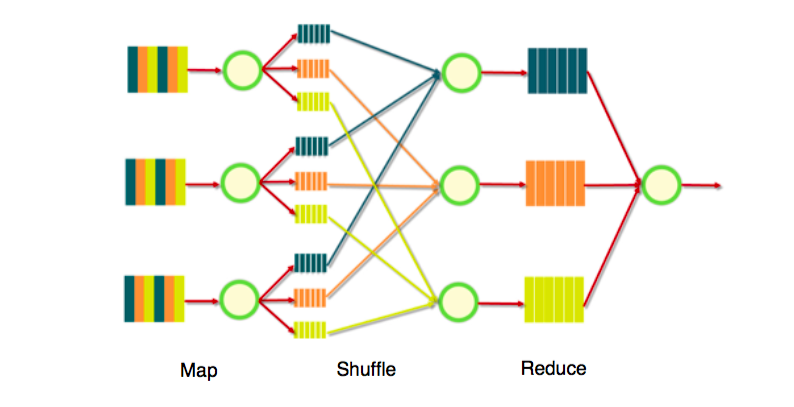
\includegraphics[scale=0.6]{image/MapRed.png}
    \caption{Схема распараллеливание.}
    \label{srg}
\end{figure}

На стадии Map параллельно считываются данные из независимых блоков, на которые
разбит исходный входной файл. Происходит их преобразование в пары (Ключ, Значение).
Затем идет стадия Shuffle: вывод функции Map распределяется по «корзинам», в
зависимости от значения ключа. Все пары (Ключ, Значение), имеющие одинаковый ключ,
попадают в одну корзину и отдаются определенному редьюсеру. Таким образом, данные
из разных частей входного файла могут собраться вместе при обработке на стадии
Reduce. Такая архитектура позволяет быстрое распараллеливание и не загружает
оперативную память, что необходимо при решении поставленной задачи.

Краткая реализация алгоритма DDM в парадигме MapReduce:

\begin{enumerate}
\item Считываются значения вектаров для каждого слова. Для первой эпохи значения
заполняются случайными величинами в диапазоне $[-0.1, 0.1]$.

\item На стадии Map происходит параллельное считывание пар $(u, v, q)$.

\item Формируется пара (Ключ, Значение) для её обработки на стадии Reduce. Ключ = $u$,
Значение = $v$. Отправляются на Reduce.

\item Для каждой такой пары генерируется $q$ негативных примеров гипонимов $u'$ и $q$
негативных примеров гиперонимов $v'$.

\item Для каждой пары $(u, v')$ ( аналогично для $(u', v)$) рассчитывается разница расстояния между $u$ и $v'$ и расстояния между $u$, $v$. Если $f(x) + \log(q) < f(x') + \log(q')$, то необходимо изменить вектора $u, v, v'$ - переход к пункту 4. Иначе просматривается следующая
пара.

\item Рассчитываются антиградиенты $du, dv, dv'$ и умножаются на шаг обучения

\item Формируются пары (Ключ, Значение) для их обработки на стадии Reduce. Ключ
соответствует самому вектору, а значение - изменению. Получаются пары $(u, du)$, $(v,
dv)$, $(v’, dv’)$. Отправляются на Reduce.

\item На стадии Reduce для каждого вектора $u$ (аналогично $v$), собирается список всех
его изменений, полученных из пункта 6 и изначальное значение вектора из пункта 1.

\item Высчитывается новое значение вектора и сохраняется в файле, для его считывания
следующий эпохой.
\end{enumerate}


\subsubsection{Тестирование}

При распараллеливании данного алгоритма на 24 кластера, получилось, что средняя
продолжительность вычисления одной эпохи составляет 50 секунд.
Параметры сети были установлены следующими: длина векора 100, шаг обучения 0.1, кол-
во эпох 100.
Также, как и при исследовании метода Word2Vec были протестированны алгоритмы GBR и
LambdaRank с видами представления векторов: $Diff, Dist1, Dist2, Cos$.
Полученные результаты:

[ТАБЛИЧКА] % исследование алгоритма 
\section{Модернизация}
\label{sec:AlgoModern_5} \index{AlgoModern_5}
\large

\subsection{Оптимизация по времени работы}
На основе результатов тестирования программы и анализа выяснилось, что эффективность алгоритма тесно связана с тем, как нумеруются вершины графа. Другими словами, время работы программы зависит от того, какой матрицей смежности (из многих) представляется граф.

Модернизация заключается в том, что на каждом этапе можно требовать, чтобы мощность множества частичных отображений была минимальна. Однако представить матрицу смежности нужным образом не представляется возможным при больших размерах, и время работы, затрачеваемой на это, превышает время работы алгоритма. Например, при $n = 100$ потребуется всего лишь 100 операций, чтобы выяснить, с какой вершины эффективнее всего начать отсчет на первой итерации. Но для того, чтобы получить выгоду на второй итерации, уже требуется более 10 000 операций [3]. Поэтому оптимальным является уменьшить только начальное множество частичных отображений.

Для получения первого множества, мощность которого будет наименьшей, в
изначальной матрице меняется порядок строк/столбцов (переименование вершин), а
именно, необходимо поменять строки и соответствующие им столбцы таким образом,
чтобы на месте первого элемента главной диагонали стояло то значение, которое встречается меньше всех других на диагонали. То есть, если на главной диагонали $70\%$ нулей и $30\%$ единиц,
необходимо поместить на первую позицию единицу. Эффективность данной модификации
исходит из того, что первая итерация алгоритма составляет множество из тех номеров
строк (столбцов), в которых значение на главной диагонали совпадает с первым
элементом главной диагонали. Значит, выбрав на эту позицию наименьший по количеству встречаний на диагонали
элемент, получается наименьшее по мощности множество.

Оценки получены для случайных матриц (вероятность нуля и единицы в каждой позиции
одинакова и равна $\frac{1}{2}$).
Предположим, что в матрице $n\times n$ на главной диагонали находится $k$ нулей, где $k \leq \frac{1}{2} n$ (если количество нулей больше половины, то за $k$ обозначается количество единиц).
Тогда, если на первое место главной диагонали выбирать элемент случайным образом,
получим, что математическое ожидание размера полученного множества будет $\frac{k}{n}*k + \frac{n-k}{n}*(n-k)$.
В модифицированном алгоритме всегда будет получаться $k$. Таким образом,
улучшение составляет $\frac{\frac{k}{n} * k + \frac{(n-k)}{n} * (n-k)} {k} = 2 \frac{k}{n} + \frac{n}{k} - 2$ раз. В случае диагонали,
состоящей из одних нулей (единиц), то есть k = 0, улучшение равняется 1 (мнощьность
множеств одинакова).
Для получения полной оценки необходимо посчитать матожидание улучшения для
произвольного числа нулей и единиц на главной диагонали. Вероятноть $k$ нулей
составляет $\frac{C_n^k}{2^n}$. Тогда матожидание улучшения $\frac{1}{2^{n-1}} + 2 \sum\limits_{i=1}^{\lceil\frac{n}{2}\rceil} \frac{C_n^k}{2^n} * (2\frac{k}{n} + \frac{n}{k} - 2)$.
Далее в таблице приведены значения для различных $n$:

\begin{tabular}[t]{||l|l||}
\hline
Количество вершин графа & Коэф. уменьшения мощности \\
\hline
4 &  2.12500 \\
\hline
8 & 2.11198 \\
\hline
14 & 1.69565 \\
\hline
20 & 1.51723 \\
\hline
50 & 1.27697 \\
\hline
100 & 1.18312 \\
\hline
200 & 1.12400 \\
\hline
\end{tabular}

\subsection{Обработка особых случаев}


\subsection{Ресурс параллелизма}
Для поиска автоморфизмов матрицы порядка $n$ итерационным алгоритмом в параллельном варианте требуется выполнить:

* $n$ ярусов сравнений (количество сравнений $ k = 1 \ldots n: \frac{1}{e^{k}} \frac{n^{n+1/2}}{(n-k-2)^{(n-k-3/2)}~2^{(k)^2}} \times (n - k)(2k + 1) $)

При классификации по высоте ЯПФ, таким образом, алгоритм имеет сложность $ O(n) $.

При классификации по ширине ЯПФ его сложность $ O(n(\frac{e}{2})^{\ln(n)^2} \ln(n))) $.
 % модернизация алгоритма
\section{Раздел 6}
\label{sec:Chapter_6} \index{Chapter_6}
\large

\subsection{Пумпумпум} % практическое применение
\section*{Заключение}
\addcontentsline{toc}{section}{Заключение}
\label{sec:Conclusion} \index{Conclusion}
\large

В данной работе были исследованы и реализованы различные методы извлечения гиперонимов из текстовых корпусов. Рассмотрен алгоритм, основанный на анализе текстов средством рукописных регулярных выражений. Протестированы шаблоны из библиотеки \textit{hearstPatterns (Python)} на текстовом корпусе UMBC и заранее извлеченные пары ProBase. Также реализованы и проанализированы алгоритмы получения векторного представления слов: Word2Vec и DDM, с последующим их дообучением алгоритмами GBR и LambdaRank. Лучшая модель протестирована на полном наборе данных с итеративным дообучением посредством выбора определенных отрицательных примеров (NegativeExample).

Наиболее удачной оказалась связка ProBase + DDM + LambdaRank + NegativeExample. ProBase обеспечивает высокой точностью, DDM увеличивает полноту, LambdaRank и NegativeExample подстраивают полученные вектора под конкретные эталонные данные. 

Полученная модель извлекает достаточно правильные гиперонимы, относительно действительных значений слов. Увеличения точности результатов на конкретных эталонных данных, позволит составление качественных шаблонов, аналогичных ProBase, на текстовом корпусе UMBC. % заключение

\nocite{*}
\bibliographystyle{utf8gost71u}
\bibliography{References}

\section*{Приложение А}
\addcontentsline{toc}{section}{Приложение А}
\label{sec:Appendix_1} \index{Appendix_1}
\large

\begin{figure}[ht]
\centering 
    %\includegraphics[scale=0.7]{image/srg_example.png}
    %\caption{Граф Пейли 13-го порядка, сильно регулярный граф с параметрами srg(13,6,2,3).}
    %\label{srg}
\end{figure}

\begin{figure}[H]
\centering
    %\includegraphics[scale=0.5]{image/program_example.jpeg}
    %\caption{Примеры использования программы}
    %\label{program_example}
\end{figure}
 % приложение
\section*{Приложение Б}
\addcontentsline{toc}{section}{Приложение Б}
\label{sec:Appendix_2} \index{Appendix_2}
\large 

Ссылка на дипломную работу с программой на github:\\
\href{https://github.com/fullincome/university}{https://github.com/fullincome/university}

Схема реализации представлена на языке C++

\begin{lstlisting}
#define GRAPH_SIZE 300
#define ROW_ARR_SIZE 10000 
#define COL_ARR_SIZE GRAPH_SIZE

const int N = GRAPH_SIZE;

vector<array<unsigned short,COL_ARR_SIZE>> 
Mi(ROW_ARR_SIZE, COL_ARR_SIZE);
vector<array<unsigned short,COL_ARR_SIZE>> 
M'i(ROW_ARR_SIZE, COL_ARR_SIZE);
unsigned char **matrix;

struct_M'i make_M'i(Mi) {
    struct_M'i M'i;
    for (auto x: Mi) {
        for (int i = 0; i < n; ++i) {
            if (check_h(x) && !eq(x, i)) {
                M'i.push_back(x.add(i));
            }
        }
    }
    return M'i;
}

struct_Mi make_Mi(M'i) {
    struct_Mi Mi;
    for (auto x: M'i) {
        for (int i = 0; i < n; ++i) {
           Mi.push_back(x.add(i));
        }
    }
    return Mi;
}

int main() {

    //fill matrix
    init_automorphisms(matrix);

    //parallelization of program
    switch(process) {
    case 0:
        begin = 0;
        end = stop_0;
    case 1:
        begin = start_1;
        end = stop_1;
    ...
    case N:
        begin = start_n;
        end = M_0.size();

    //main cycle
    for (i = begin; i < end; ++i) {
        Mi = make_Mi(M'i-1);
        M'i = make_M'i(Mi);
    }

    //results save (automorphisms output)
    final_automorphism(M'i);
}
\end{lstlisting}
 % приложение


\end{document}
